\section{Leben aus Stickstoff – die Zukunft der Ammoniakproduktion}
\sectionmark{N2-Reduktion}

%\begin{figurehere}
%	\begin{center}
%		\includegraphics[width=\linewidth]{Bilder/andechs2.jpg}
%%		\caption{xxx} 
%	\end{center}
%\end{figurehere}

\begin{multicols}{2}	
Das Stickstoff-Atom ist einer der Grundbausteine lebendiger Materie. Mikroorganismen fixieren den in molekularer Form (N2) vorliegenden Luftstickstoff und machen ihn nutzbar für die Bildung von Proteinen und anderen Biomolekülen. Wie auch für Sauerstoff oder Kohlendioxid hat sich im Zuge der Entwicklung des Lebens ein komplexer Stickstoff-Kreislauf auf der Erde ausgebildet. Spätestens seit der Entwicklung des Haber-Bosch-Verfahrens zu Beginn des 19. Jahrhunderts greift die Menschheit in industriellem Maßstab in diesen Kreislauf ein. Zur Ernährung der wachsenden Weltbevölkerung wird in gigantischen Mengen Ammoniak (NH3) synthetisiert, der als Ausgangsstoff für pflanzlichen Dünger dient. Durch die Reaktivität des Ammoniak-Moleküls wird der darin enthaltene Stickstoff für organische Synthesen nutzbar – anders als im molekularen Stickstoff, dessen energetisch günstige Dreifachbindung extrem stabil und schwer aufzuspalten ist. Die energetisch aufwendige Fixierung des Luftstickstoffs wird der Natur damit gewissermaßen abgenommen, und Nutzpflanzen können schneller und dichter wachsen, als die natürliche Bodenverfügbarkeit von fixiertem Stickstoff es erlauben würde. Dies ist seit dem 20. Jahrhundert eine notwendige Voraussetzung für die Ernährung der rasant gewachsenen Weltbevölkerung.
\\
Über die Risiken, die mit der massiven Beeinflussung des globalen Stickstoffkreislaufes einhergehen, ist in der breiten Gesellschaft kaum etwas bekannt – die Verankerung entsprechender Forschungsergebnisse im kollektiven Denken und Handeln erleben wir gerade erst im Bezug auf anthropogene CO2- und Treibhausgas-Emissionen. Doch auch hier schon spielt die globalen Ammoniak-Produktion, bedingt durch ihre enormen Ausmaße, eine elementare Rolle. Die Herstellung der jährlich verbrauchten über 100 Megatonnen Ammoniak beansprucht 2\% der gesamten weltweiten Energieproduktion und verbraucht 3-5\% der jährlich geförderten Erdgasmenge. Damit einher geht ein signifikanter Beitrag zu den globalen CO2-Emissionen, und damit zum menschengemachten Klimawandel. Wer sich davon nicht behelligen lässt, ist vielleicht für ein geopolitisches Argument empfänglicher: Das bislang alternativlose Haber-Bosch-Verfahren zur industriellen Ammoniak-Herstellung ist wegen der erforderlichen hohen Temperaturen und Drücke nur in großtechnischen Anlagen wirtschaftlich realisierbar. Die Zentralisierung der Produktion, inklusive einer darauf ausgerichteten Infrastruktur, hat heutzutage ein globales Ausmaß. 30\% der globalen Ammoniak-Produktion erfolgen in China, danach kommen mit je 8-10\% die USA, die EU, Indien, Russland und der nahe Osten. Da die Produktion auf Erdgas angewiesen ist, ist dessen billige Verfügbarkeit eine Voraussetzung. Damit kann der Export von Ammoniak und abgeleiteten Produkten nur allzu leicht ein Spielball geopolitischer Interessen werden.
\\
Die Chancen alternativer Herstellungsverfahren liegen nun auf der Hand. Eine dezentrale Produktion ohne Abhängigkeit von Erdgas könnte, großflächig umgesetzt, die Energiewende unterstützen und die Souveränität von Verbraucherländern stärken. Dazu kommen bei einer verbrauchernahen Erzeugung die eingesparten Emissionen, die durch den weltweiten Transport anfallen. Welche Möglichkeiten gibt es? Für die nächsten 20 bis 30 Jahre wird ein „grünes“ Haber-Bosch-Verfahren die größte industrielle Bedeutung haben, bei dem der notwendige Wasserstoff durch Elektrolyse (mit Strom aus erneuerbaren Quellen) statt durch die Verarbeitung von Erdgas bereitgestellt wird. Für die Zeit danach werden mehrere, bislang leider nicht skalierbare Lösungen erforscht. Von der Natur inspirierte künstliche Enzyme, lithiumhaltige Elektrolytlösungen, durch Sonneneinstrahlung beheizte Reaktoren – das Spielfeld ist weit. Fest steht, dass eine neue Art der Ammoniaksynthese unsere Gesellschaft und unsere Wirtschaft prägen wird, ebenso, wie es der Haber-Bosch-Prozess die letzten hundert Jahre getan hat.
\\
Zum Schluss ein paar Worte zu meiner Verbindung mit diesem Thema: Im Rahmen meiner Doktorarbeit am Walter-Schottky-Institut der Technischen Universität München erforsche ich Halbleitermaterialien, die wie Solarzellen Energie in Form von angeregten Elektronen bereitstellen können. Ich versuche, mit diesen Elektronen die Reduktion von Stickstoff zu Ammoniak in Wasser anzutreiben. Würde dieser Ansatz funktionieren, böte er eine gut skalierbare Lösung, ähnlich wie die Brennstoffzelle zur Wasserstofferzeugung. Momentan tragen unsere Bemühungen keinen Erfolg, aber ich bin gespannt, was die nächsten 3 Jahre noch bringen werden. Über dieses Thema gibt es noch vieles zu berichten, und gerne empfehle ich weiterführende Artikel.
\\
Die Geschichte des Haber-Bosch-Prozesses und der namensgebenden Wissenschaftler ist mit ihren vielen historischen Verflechtungen und ihrer moralischen Ambivalenz eine unbedingte Empfehlung zur persönlichen Weiterbildung. Die künstliche Ammoniaksynthese brachte im ersten Jahrhundert ihrer Erfindung Leben und Tod für Hunderte Millionen von Menschen. Wir dürfen hoffen, dass sie im folgenden Jahrhundert ein beispielhafter Erfolg auf dem Weg der ökologischen und wirtschaftlichen Transformation unserer Gesellschaft wird.
\\
\begin{flushright}
		\hfill\emph{Maximilian Christis Va!}
	\end{flushright}
		
\end{multicols}


\begin{figurehere}
	\begin{center}
		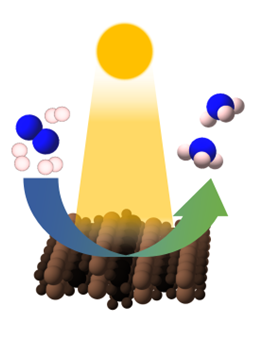
\includegraphics[width=.4\linewidth]{./Bilder/2.0.Stickstoff_Reduktion/Bild1.png} \caption{Prozess der photochemischen Ammoniak-Synthese an der Oberfläche eines Katalysators.} 
	\end{center}
\end{figurehere}



\begin{figurehere}
	\begin{center}
		 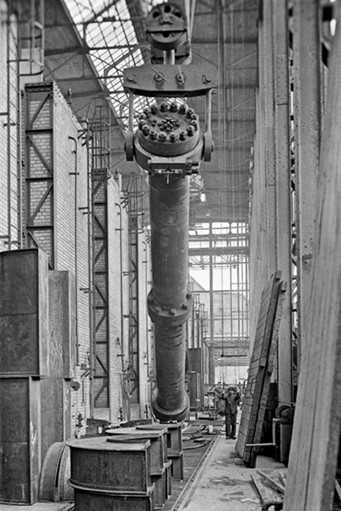
\includegraphics[width=.4\linewidth]{./Bilder/2.0.Stickstoff_Reduktion/Bild2.jpg} 
		 \caption{Erster Haber-Bosch-Reaktor im BASF-Werk Oppau, 1913. © BASF}
	\end{center}
\end{figurehere}


%
%\begin{figurehere}
%	\begin{center}
%		\includegraphics[width=.8\linewidth]{Bilder/pios2}
%		\caption{Realer Aufbau} 
%	\end{center}
%\end{figurehere}